\section{Problema y algoritmos de filtraje}
Se considera un sistema controlado-observado estocástico a tiempo discreto
\begin{align*}
	\mathbf{x}_{k+1} &= \mathbf{f}(t_k, \mathbf{x}_k, \mathbf{u}_k, \mathbf{w}_k) \\
	\mathbf{y}_k &= \mathbf{g}(t_k, \mathbf{x}_k, \mathbf{u}_k, \mathbf{v}_k)
\end{align*}
Donde:
\begin{itemize}
	\item $\mathbf{f}: \R \times \R^{n_x} \times \R^{n_u} \times \R^{n_w} \to \R^{n_x}$ es la función de dinámica.
	\item $\mathbf{g}: \R \times \R^{n_x} \times \R^{n_u} \times \R^{n_v} \to \R^{n_y}$ es la función de observación.
\end{itemize}
Siendo $n_x$ la dimensión del estado, $n_y$ la dimensión de la observación, $n_u$ la dimensión del \textit{input}, $n_w$ la dimensión del proceso estocástico en la dinámica y $n_v$ la dimensión del ruido en las observaciones. Se considera una condición inicial $\mathbf{x}_0$, por lo general desconocida sobre la que se coloca un \textit{prior} $X_0$. 

Se supondrá que tanto $\mathbf{v}_k$ como $\mathbf{w}_k$ son vectores aleatorios centrados tal que $\mathbf{w}_k \indep \mathbf{w}_m, \, \forall k \neq m$, $\mathbf{v}_k \indep \mathbf{v}_m, \, \forall k \neq m$ y $\mathbf{w}_k \indep \mathbf{v}_k, \, \forall k$. Se dirá que $\mathbf{w}$ y $\mathbf{v}$ son la perturbación en la dinámica y ruido en la medición, respectivamente. 

El estudio de sistemas a tiempo continuo, formulados como
\begin{align*}
	\mathbf{x}'(t) &= \mathbf{f}(t, \mathbf{x}(t), \mathbf{u}(t), \mathbf{w}(t)) \\
	\mathbf{y}(t) &= \mathbf{g}(t, \mathbf{x}(t), \mathbf{u}(t), \mathbf{v}(t))
\end{align*}
muchas veces se reduce al caso discreto con esquemas de tipo Euler, por lo que durante esta tesis se mantendrá el foco en sistemas a tiempo discreto.

El objetivo en el caso discreto será, en un instante $k$ encontrar un estimador de $\mathbf{x}_{k+\alpha}$, en base a observaciones $\{\mathbf{y}_k\}_k$, que será denotado por $\hat {\mathbf{x}}_{k+\alpha}$. Dependiendo del valor de $\alpha$ el algoritmo recibirá una categoría diferente:
\begin{itemize}
	\item Predicción: $\alpha > 0$.
	\item Filtraje: $\alpha = 0$.
	\item Suavizado: $\alpha < 0$.
\end{itemize}
Así también se denotará a $\hat {\mathbf{x}}_{k_1|k_2}$ a la estimación del estado en la iteración $k_1$ dadas mediciones hasta la iteración $k_2$, entonces se dirá que $\hat{\mathbf{x}}_{k_1 | k_2}$ es un estado
\begin{itemize}
	\item Suavizado, si $k_2 > k_1$ ($t_2 > t_1$).
	\item Filtrado, si $k_2 = k_1$ ($t_2 = t_1$).
	\item Predicho, si $k_1 > k_2$ ($t_1 > t_2$).
\end{itemize}
El caso del filtraje será el centro durante este trabajo. Un algoritmo de filtraje busca estimar en el tiempo presente el estado en base a observaciones ruidosas, que puede ser entendido como el primer proceso en la estimación del estado de un sistema. 

Posterior al filtraje de una medición ruidosa, se siguen los procesos de predicción y/o suavizado, siendo el primero la tarea poder estimar estados futuros en base al pasado, sin información del momento a estimar. Mientras que el suavizado es la capacidad de estimar momentos pasados, lo que se utiliza para mejorar las estimaciones presentes.

Se denota por $\mathbf{y}_{1:k}$, $\mathbf{u}_{0:k}$ a las observaciones e \textit{inputs}, respectivamente, hasta el tiempo $k \in \N$, a $k \in \N$ le llamaremos el horizonte del problema.  Notar que se considerará que no se tiene una observación de la condición inicial.

El problema de filtraje se puede formular como un problema de optimización del error cuadrático medio de la estimación, condicional a las observaciones y a los \textit{inputs}
\begin{equation*}
	(P) \quad
	\begin{cases}
		\begin{aligned}
			\text{mín} \quad & \quad \sum_{k=0}^N \E \left [ (\hat{\mathbf{x}}_{k|k} - \mathbf{x}_k)^T(\hat{\mathbf{x}}_{k|k} - \mathbf{x}_k) | \mathbf{y}_{1:k}, \, \mathbf{u}_{0:k}  \right] \\ 
			\text{s.a} \quad & \quad \mathbf{x}_{k+1} = \mathbf{f}(t_k, \mathbf{x}_k, \mathbf{u}_k, \mathbf{w}_k) \\
			\text{} \quad & \quad \mathbf{y}_k = \mathbf{g}(t_k, \mathbf{x}_k, \mathbf{u}_k, \mathbf{v}_k) \\
			\text{} \quad & \quad \mathbf{x}_0 \sim X_0
		\end{aligned}
	\end{cases}
\end{equation*}
Es entonces que el problema $(P)$ tiene como solución al estimador de mínimo error cuadrático. Es sabido de \cite{Kalman1960AProblems, Setoodeh2022NonlinearApplications} que este problema tiene un óptimo global dado por la esperanza condicional, que coincide con la noción de dicho estimador.
\begin{prop}
	El óptimo de $(P)$ viene dado por 
	\begin{equation*}
		\hat{\mathbf{x}}_{k|k} = \E \left [ \mathbf{x}_k | \mathbf{y}_{1:k}, \, \mathbf{u}_{0:k}  \right], \quad \forall k \in \{ 0, \dots, N \}
	\end{equation*}
\end{prop}
\noindent Aunque dicha cantidad no sea computable por métodos clásicos, como Monte Carlo, existen algoritmos para poder calcularla tiempo a tiempo, aunque sea de manera aproximada. 
\subsection{Caso a tiempo discreto, dinámica lineal y ruido centrado}
Para abordar el caso de sistemas dinámicos controlados-observados generales, es importante estudiar primero el caso lineal, con ruidos centrados y segundo momento finito, esto es
\begin{equation}
	\begin{cases}
		\mathbf{x}_{k+1} &= \mathbf{A}_k \mathbf{x}_k + \mathbf{B}_k \mathbf{u}_k + \mathbf{w}_k \\
		\mathbf{y}_k &= \mathbf{C}_k \mathbf{x}_k + \mathbf{D}_k \mathbf{u}_k  + \mathbf{v}_k
	\end{cases}
	\label{eq:lin_disc}
\end{equation}
con $\mathbf{A}_k \in \R^{n_x \times n_x}$, $\mathbf{B}_k \in \R^{n_x \times n_u}$, $\mathbf{C}_k \in \R^{n_y \times n_x}$, $\mathbf{D}_k \in \R^{n_y \times n_u}$, $\E[\mathbf{w}_k] = 0$, $\text{Cov}(\mathbf{w}_k) = \mathbf{Q}_k$, $\E[\mathbf{v}_k] = 0$, $\text{Cov}(\mathbf{v}_k) = \mathbf{R}_k$, $\mathbf{Q}_k \in \R^{n_x \times n_x}$, $\mathbf{R}_k \in \R^{n_y \times n_y}$ matrices de covarianza. Se tiene un algoritmo muy utilizado en ingeniería y ciencia, con suficiente fundamentos matemáticos e implementaciones eficientes, denotado el filtro de Kalman en honor a Rudolf E. Kalman, quién propuso el algoritmo por primera vez en \cite{Kalman1960AProblems}. Los detalles del algoritmo se presentan en el pseudo-código del Algoritmo \ref{alg:KF}. 
\begin{algorithm}
	\caption{Filtro de Kalman}\label{alg:KF}
	\begin{algorithmic}[1]
		\State \textbf{Entrada:} Dinámica discreta como en (\ref{eq:lin_disc}), $\mathbf{x}_0$ \textit{prior} sobre la condición inicial, $\mathbf{y}_{1:N}$ observaciones, $\mathbf{u}_{0:N}$ \textit{inputs}.
		\State \textbf{Salida:} $(\hat{\mathbf{x}}_{k|k})_{k=0}^{N}$ estimador de la trayectoria y $(\hat{\mathbf{P}}_{k|k})_{k=0}^{N}$ matrices de covarianza.
		\State $\hat{\mathbf{x}}_{0|0}   \gets \E [\mathbf{x}_0]$
		\State $\mathbf{P}_{0|0} \gets \E [(\mathbf{x}_0 - \hat{\mathbf{x}}_{0})(\mathbf{x}_0 - \hat{\mathbf{x}}_{0})^T]$
		\For{$k = 0, \dots, N-1$}
		\State $\hat{\mathbf{x}}_{k+1|k} \gets \mathbf{A}_k \mathbf{x}_{k|k} + \mathbf{B}_k \mathbf{u}_k$
		\Comment{Estimación a priori}
		\State $\mathbf{P}_{k+1|k} \gets \mathbf{A}_k \mathbf{P}_{k|k} \mathbf{A}_k^T + \mathbf{Q}_k$
		\Comment{Error de covarianza a priori}
		\State $\hat{\mathbf{y}}_{k+1|k} \gets \mathbf{C}_{k+1} \hat{\mathbf{x}}_{k+1|k}$ 
		\Comment{Estimación de observación a priori}
		\State $\mathbf{e}_{\mathbf{y}_{k+1|k}} \gets \mathbf{y}_{k+1} - \hat{\mathbf{y}}_{k+1|k}$
		\Comment{Error a priori (innovación)}
		\State $\mathbf{K}_{k+1} \gets \mathbf{P}_{k+1|k} \mathbf{C}^T_{k+1} (\mathbf{C}_{k+1} \mathbf{P}_{k|k} \mathbf{C}^T_{k+1}+ \mathbf{R}_{k+1})^{-1}$
		\Comment{Ganancia de Kalman}
		\State $\hat{\mathbf{x}}_{k+1|k+1} \gets \hat{\mathbf{x}}_{k+1|k} + \mathbf{K}_{k+1} \mathbf{e}_{\mathbf{y}_{k+1|k}}$
		\Comment{Error a posteriori}
		\State $\mathbf{P}_{k+1|k+1} \gets (\mathbf{I} - \mathbf{K}_{k+1} \mathbf{C}_{k+1}) \mathbf{P}_{k+1|k}$
		\Comment{Error de covarianza a posteriori}
		\EndFor
	\end{algorithmic}
\end{algorithm}\\
El siguiente resultado le da toda su validez al algoritmo del Filtro de Kalman, que es probado en el artículo original \cite{Kalman1960AProblems}.
\begin{prop}
	El algoritmo del filtro de Kalman devuelve una secuencia $(\hat{\mathbf{x}}_{k|k})_k$ tal que 
	\begin{equation*}
		\hat{\mathbf{x}}_{k|k} = \E \left [ \mathbf{x}_k | \mathbf{y}_{1:k}, \, \mathbf{u}_{0:k}  \right], \quad \forall k \in \{ 0, \dots, N \}
	\end{equation*}
\end{prop}
\noindent Como consecuencia del hecho de que en el contexto Gaussiano el estimador de mínimo error cuadrático medio coincide con el estimador de máximo a posteriori, se tiene el siguiente resultado.
\begin{prop}
	Si además $\mathbf{w}_k \sim \mathcal{N}(0, \mathbf{Q}_k)$ y $\mathbf{v}_k \sim \mathcal{N}(0, \mathbf{R}_k)$, entonces el algoritmo del filtro de Kalman devuelve una secuencia $(\hat{\mathbf{x}}_{k|k})_k$ tal que 
	\begin{equation*}
		\hat{\mathbf{x}}_{k|k} \in \arg \max_{\hat{\mathbf{x}}_{k|k}} p (\hat{\mathbf{x}}_{k|k} | \mathbf{y}_{1:k}, \, \mathbf{u}_{0:k})
	\end{equation*}
\end{prop}

El algoritmo del Filtro de Kalman sigue un procedimiento de predicción y actualización:
\begin{itemize}
    \item Predicción: $\hat{\mathbf{x}}_{k|k} \to \hat{\mathbf{x}}_{k+1|k}$, donde solo es considerada la dinámica.
    \item Actualización: $\hat{\mathbf{x}}_{k+1|k} \to \hat{\mathbf{x}}_{k+1|k+1}$, donde se corrige la predicción en base a las observaciones.
\end{itemize}
Esta será la base para el resto de algoritmos. Para visualizar el comportamiento del algoritmo se dejan los siguientes diagramas, en donde se tiene un estado real o subyacente, en azul, y se le entrega al algoritmo una observación ruidosa, en amarillo.
\begin{itemize}
    \item Primera iteración: se comienza con un punto que, eventualmente está lejos de la condición inicial real del sistema, y luego se hace el proceso de predicción y actualización.
    \begin{figure}[h!]
        \centering
        \begin{subfigure}[b]{.49\linewidth}
        \centering
            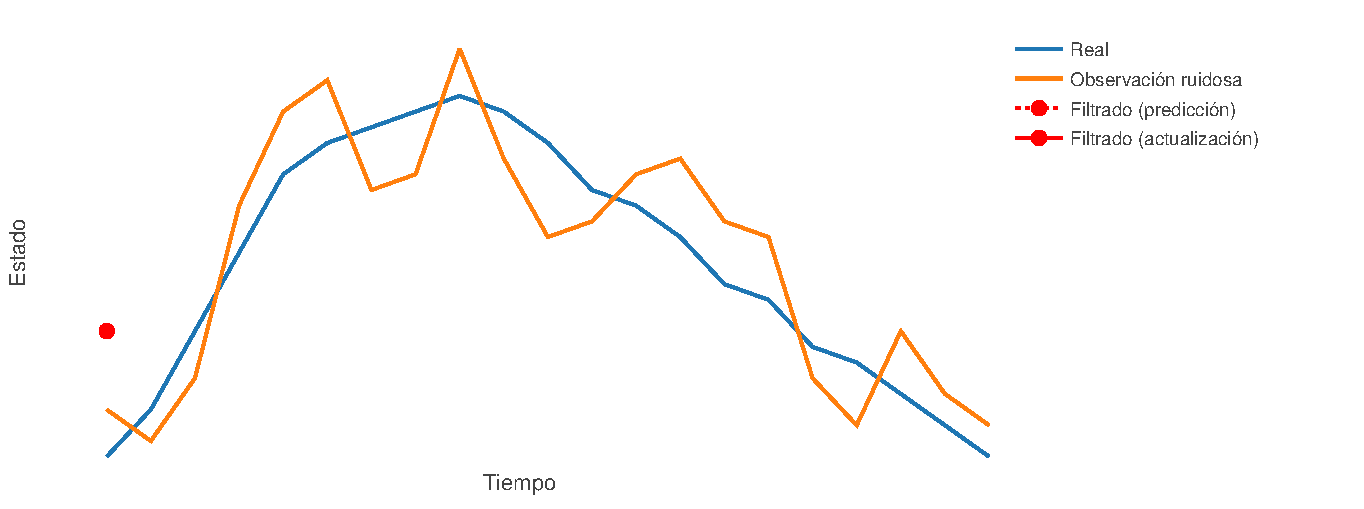
\includegraphics[width=\linewidth]{img/content/chapter2/filt0.pdf}
            \caption{Condición inicial de la iteración.}
        \end{subfigure}
        \begin{subfigure}[b]{.49\linewidth}
        \centering
            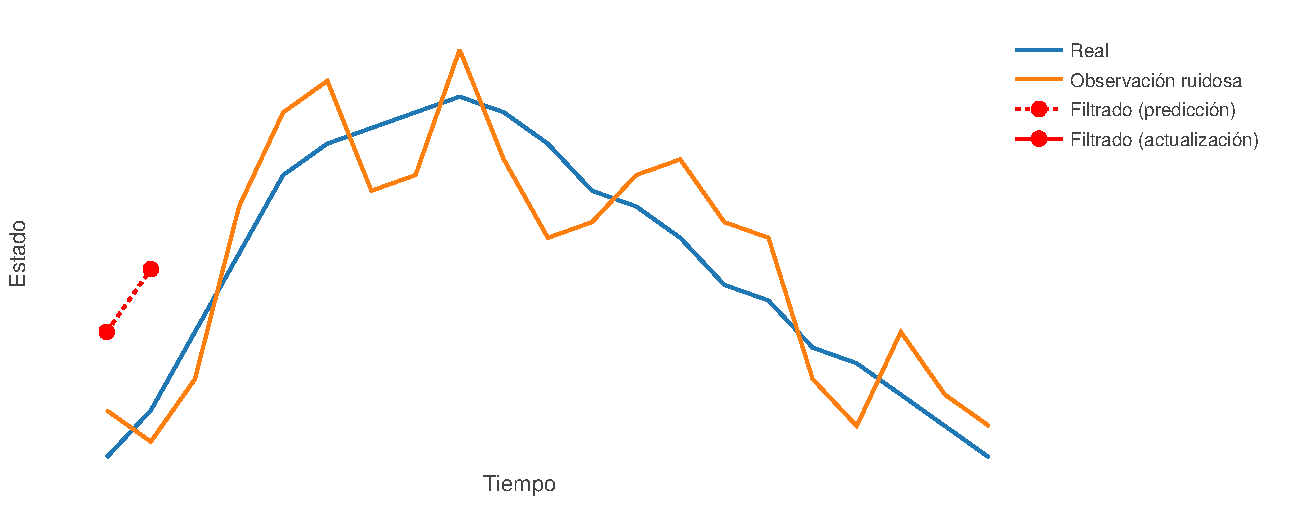
\includegraphics[width=\linewidth]{img/content/chapter2/filt1.pdf}
            \caption{Predicción.}
        \end{subfigure}
        \begin{subfigure}[b]{.49\linewidth}
        \centering
            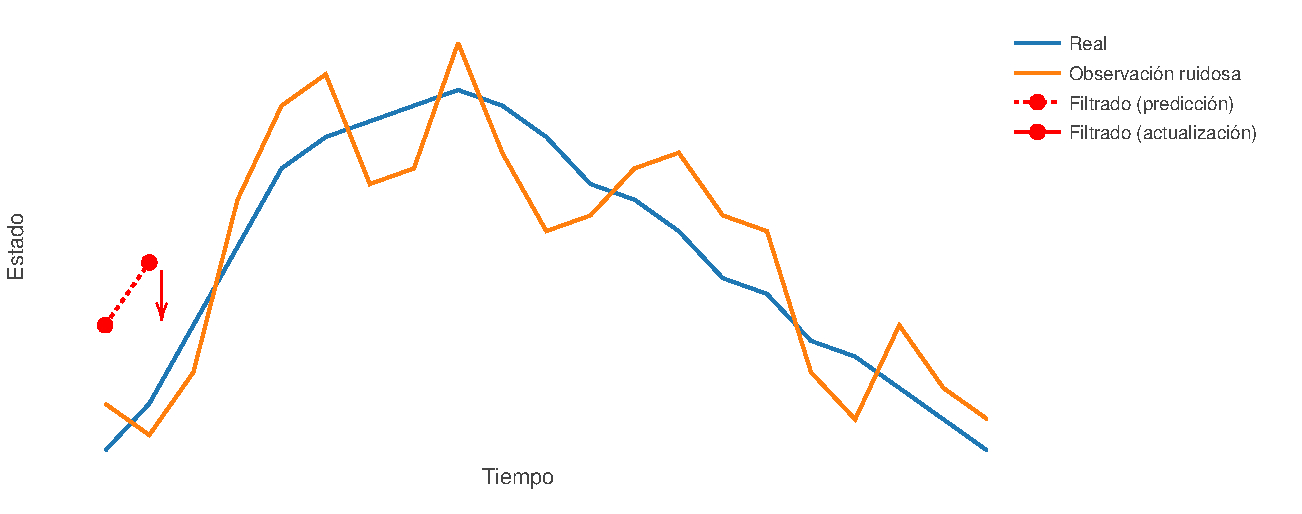
\includegraphics[width=\linewidth]{img/content/chapter2/filt2.pdf}
            \caption{Elección de la dirección de proyección.}
        \end{subfigure}
        \begin{subfigure}[b]{.49\linewidth}
        \centering
            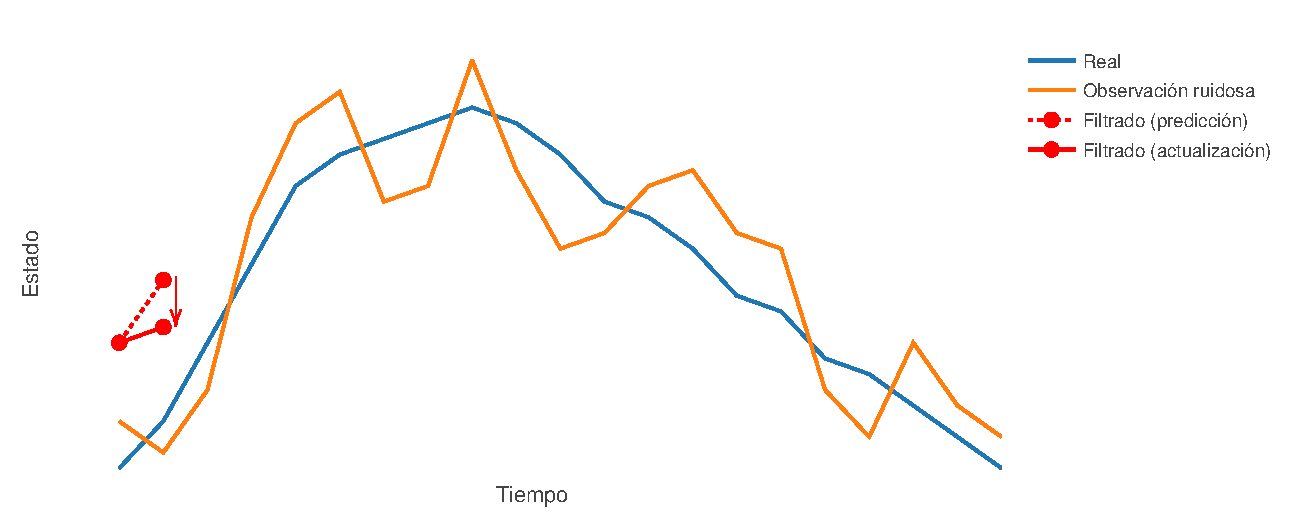
\includegraphics[width=\linewidth]{img/content/chapter2/filt3.pdf}
            \caption{Proyección.}
        \end{subfigure}
        \caption{Primera iteración de un algoritmo de filtraje.}
    \end{figure}
    \item Segunda iteración: comenzando desde el mismo punto en donde terminó la iteración anterior se observa que el estado filtrado se acerca al estado real o subyacente.
        \begin{figure}[h!]
        \centering
        \begin{subfigure}[b]{.49\linewidth}
        \centering
            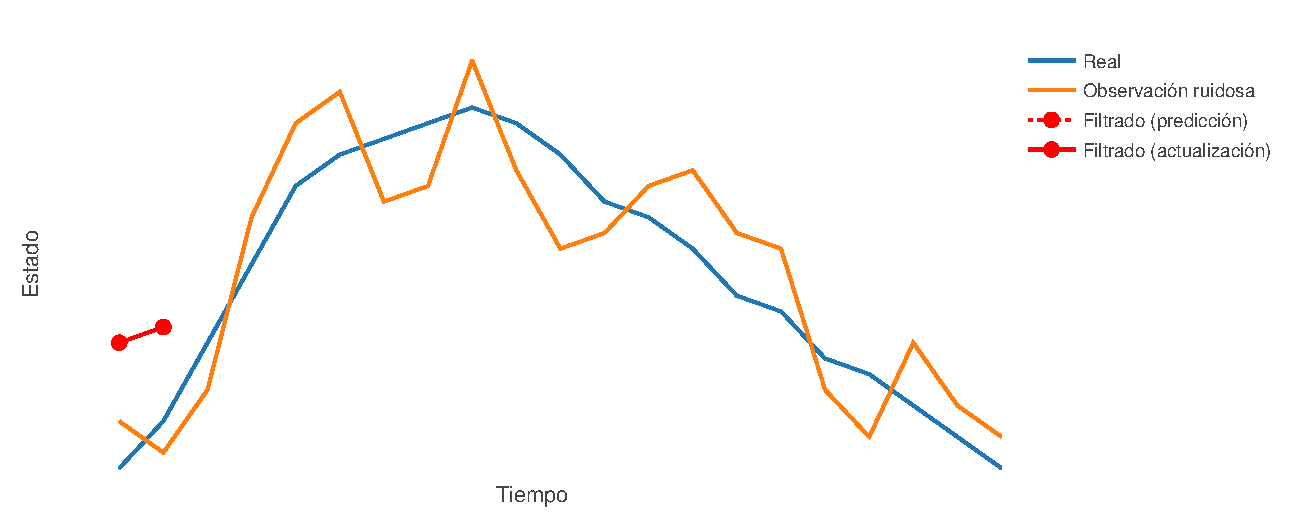
\includegraphics[width=\linewidth]{img/content/chapter2/filt4.pdf}
            \caption{Condición inicial de la iteración.}
        \end{subfigure}
        \begin{subfigure}[b]{.49\linewidth}
        \centering
            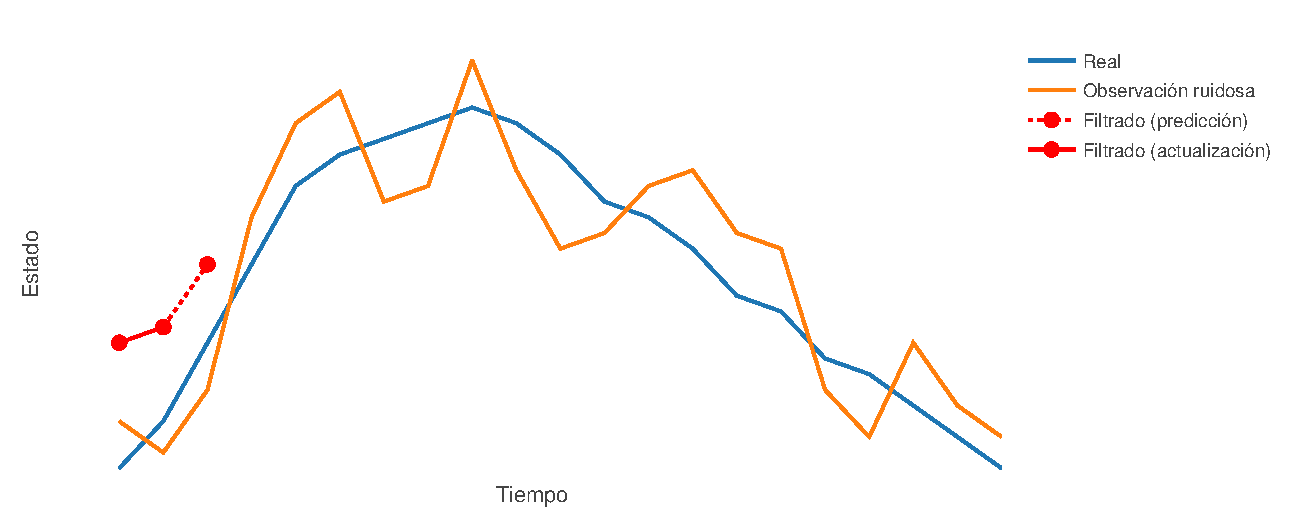
\includegraphics[width=\linewidth]{img/content/chapter2/filt5.pdf}
            \caption{Predicción.}
        \end{subfigure}
        \begin{subfigure}[b]{.49\linewidth}
        \centering
            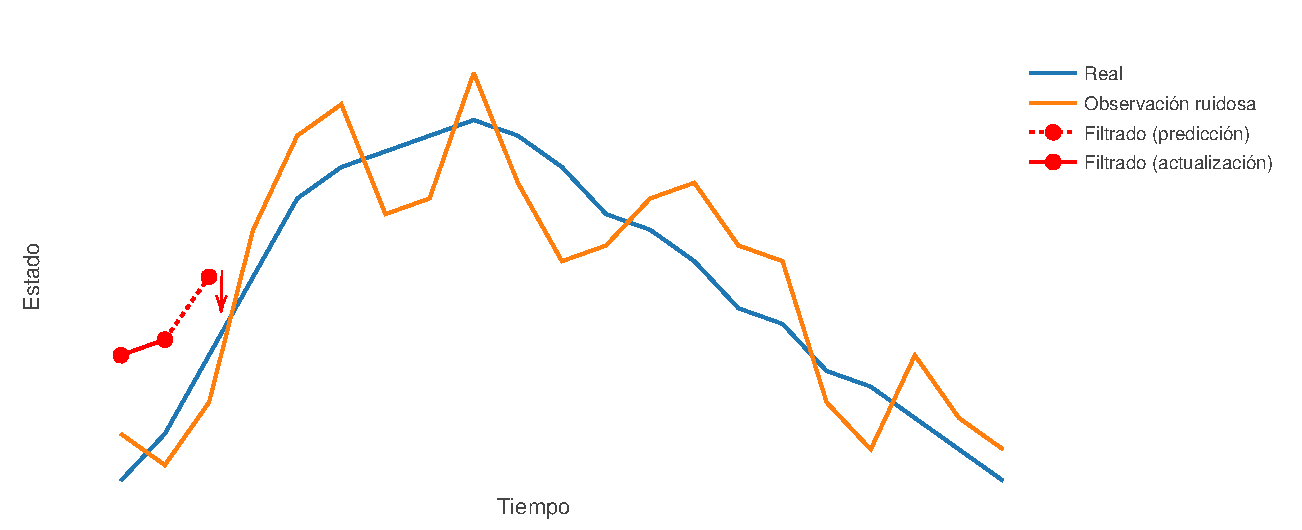
\includegraphics[width=\linewidth]{img/content/chapter2/filt6.pdf}
            \caption{Elección de la dirección de proyección.}
        \end{subfigure}
        \begin{subfigure}[b]{.49\linewidth}
        \centering
            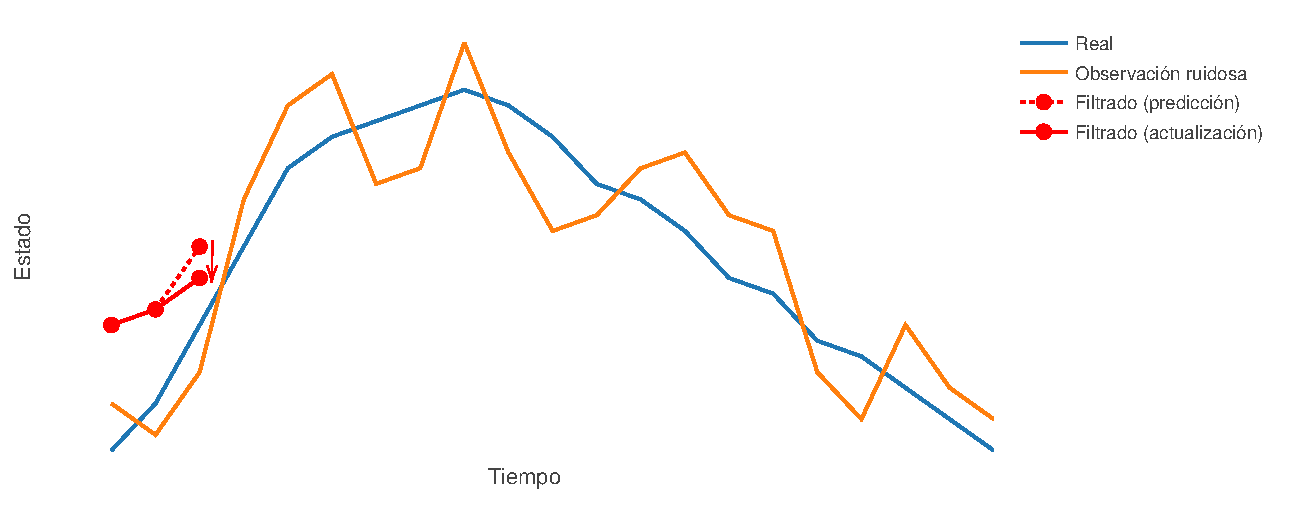
\includegraphics[width=\linewidth]{img/content/chapter2/filt7.pdf}
            \caption{Proyección.}
        \end{subfigure}
        \caption{Segunda iteración de un algoritmo de filtraje.}
    \end{figure}
    \item Iteraciones futuras: se espera que el estado filtrado ya sea muy cercano, eventualmente idéntico, al estado subyacente, con lo que se dice que el filtro se estabiliza.
    \begin{figure}[h!]
        \centering
        \begin{subfigure}[b]{.49\linewidth}
        \centering
            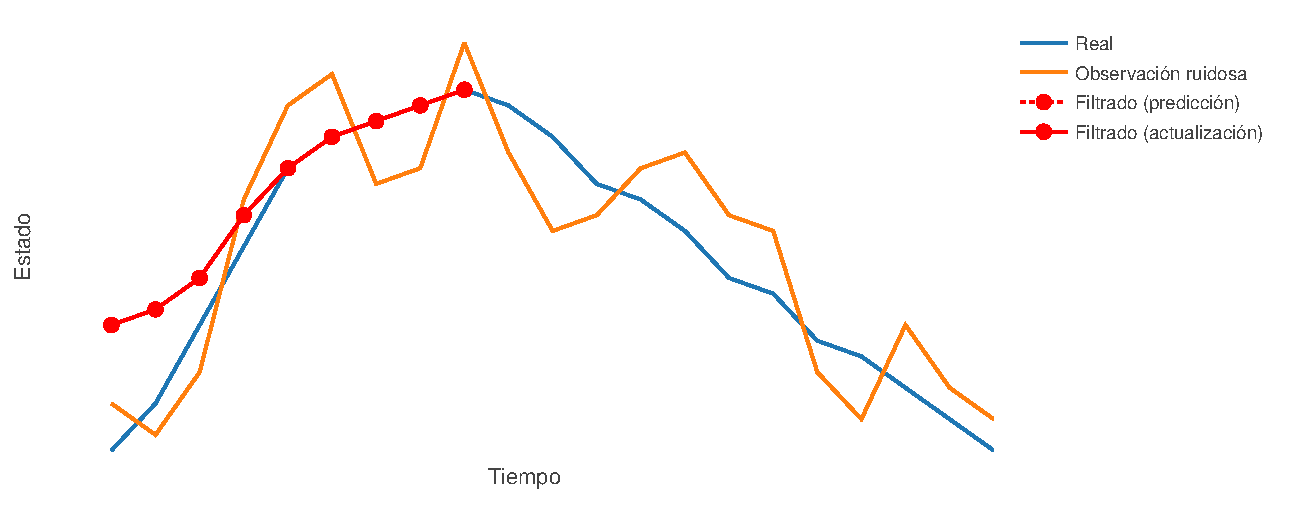
\includegraphics[width=\linewidth]{img/content/chapter2/filt25.pdf}
            \caption{$k$-ésima iteración.}
        \end{subfigure}
        \begin{subfigure}[b]{.49\linewidth}
        \centering
            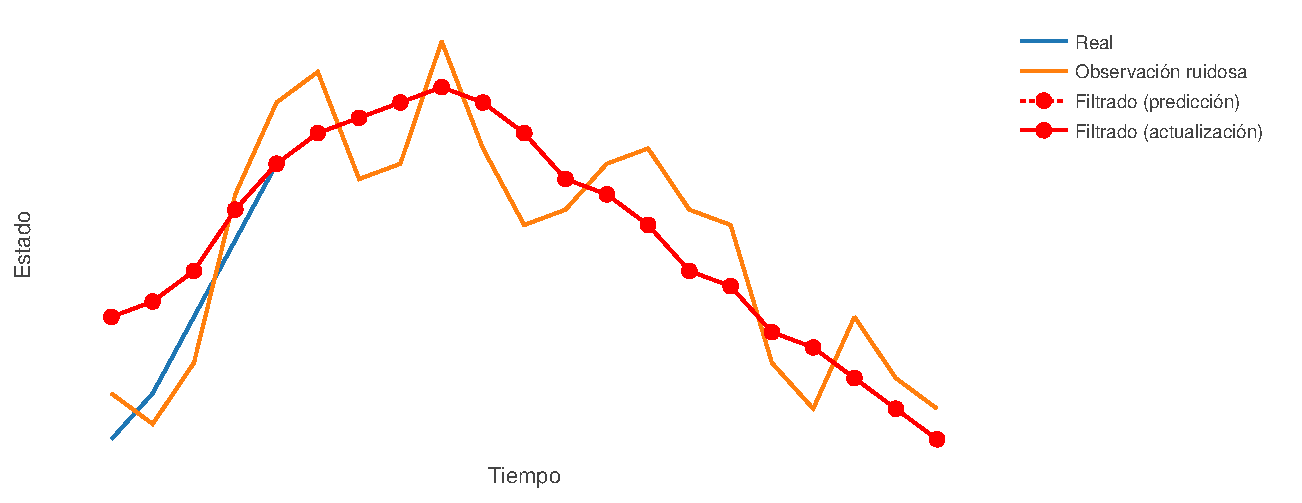
\includegraphics[width=\linewidth]{img/content/chapter2/filt26.pdf}
            \caption{Última iteración.}
        \end{subfigure}
        \caption{Últimas iteraciones de un algoritmo de filtraje.}
    \end{figure}
\end{itemize}

\subsection{Caso a tiempo discreto no lineal general}
En paralelo a los trabajos de Kalman para el caso lineal, Stratonovich estudió el caso no lineal general \cite{Stratonovich1959OptimumNoise, Stratonovich1965ApplicationSignals.} en donde el problema se reduce a la solución de una ecuación diferencial estocástica cuya solución coincide con el resultado de Kalman para el tiempo discreto y Kalman y Bucy para tiempo continuo \cite{Kalman1961NewTheory}. Pero, para el caso más general posible Maurel y Michel \cite{Maurel1984DesFinie} probaron que las soluciones de la ecuación de Stratonovich poseen una representación infinito dimensional, lo que las hace imposible de representar en un computador, lo que obliga a buscar aproximaciones.
Los primeros aprontes al caso no lineal fueron el \textit{Extended Kalman Filter} (EKF) \cite{Smith1962ApplicationVehicle, McElhoe1966AnVenus} y el \textit{Unscented Kalman Filter} (UKF) \cite{Julier2004UnscentedEstimation}, pero se sabe que resultan ser subóptimos \cite{Setoodeh2022NonlinearApplications}.\\ 
Para esta sección, se supondrá que la dinámica es de la forma
\begin{equation}
	\begin{aligned}
		\mathbf{x}_{k+1} &= \mathbf{f}(t_k, \mathbf{x}_k, \mathbf{u}_k) + \mathbf{w}_k \\
		\mathbf{y}_k &= \mathbf{g}(t_k, \mathbf{x}_k, \mathbf{u}_k) + \mathbf{v}_k 
	\end{aligned}
	\label{eq:no_lin_disc_add}
\end{equation} 
con $\E[\mathbf{w}_k] = 0$, $\text{Cov}(\mathbf{w}_k) = \mathbf{Q}_k$, $\E[\mathbf{v}_k] = 0$, $\text{Cov}(\mathbf{v}_k) = \mathbf{R}_k$. 
El algoritmo de \textit{Extended Kalman Filter}, cuyo pseudo-código puede visualizarse en el algoritmo \ref{alg:EKF}, busca linearizar el sistema a primer orden vía su Jacobiano, tanto para $\mathbf{f}$ como para $\mathbf{g}$, de manera de generar las matrices $\mathbf{A}_k$ y $\mathbf{C}_k$ necesarias para el Filtro de Kalman, respectivamente. \\
A pesar de los simple que parece la adaptación de este algoritmo al caso no lineal, ilustra que extender el filtro de Kalman al caso no lineal se basa en una linealización de la dinámica, en este caso vía Jacobiano, pero podrían existir otras, que es en lo que se basará el filtro creado durante este trabajo.

\begin{algorithm}
	\caption{\textit{Extended Kalman Filter}}\label{alg:EKF}
	\begin{algorithmic}[1]
		\State \textbf{Entrada:} Dinámica discreta como en (\ref{eq:no_lin_disc_add}), $\mathbf{x}_0$ \textit{prior} sobre la condición inicial,  $\mathbf{y}_{1:N}$ observaciones, $\mathbf{u}_{0:N}$ \textit{inputs}.
		\State \textbf{Salida:} $(\hat{\mathbf{x}}_{k|k})_{k=0}^{N}$ estimador de la trayectoria y $(\hat{\mathbf{P}}_{k|k})_{k=0}^{N}$ matrices de covarianza.
		\State $\hat{\mathbf{x}}_{0|0}   \gets \E [\mathbf{x}_0]$
		\State $\mathbf{P}_0 \gets \E [(\mathbf{x}_0 - \hat{\mathbf{x}}_{0})(\mathbf{x}_0 - \hat{\mathbf{x}}_{0})^T]$
		\For{$k = 0, \dots, N-1$}
		\State $\mathbf{A}_k \gets \nabla _\mathbf{x} \mathbf{f} (t_k, \hat{\mathbf{x}}_{k|k}, \mathbf{u}_k)$
		\Comment{Linealización de la función de dinámica}
		
		\State $\hat{\mathbf{x}}_{k+1|k} \gets \mathbf{f}(t_k, \hat{\mathbf{x}}_{k|k}, \mathbf{u}_k)$
		\Comment{Estimación a priori}
		\State $\mathbf{P}_{k+1|k} \gets \mathbf{A}_k \mathbf{P}_{k|k} \mathbf{A}_k^T + \mathbf{Q}_k$
		\Comment{Error de covarianza a priori}
		\State $\mathbf{C}_{k+1} \gets \nabla_\mathbf{x} \mathbf{g} (t_k, \hat{\mathbf{x}}_{k+1|k}, \mathbf{u}_k)$
		\Comment{Linealización de la función de observación}
		\State $\hat{\mathbf{y}}_{k+1|k} \gets \mathbf{g}(t_k, \hat{\mathbf{x}}_{k+1|k}, \mathbf{x}_{k+1})$ 
		\Comment{Estimación de observación a priori}
		\State $\mathbf{e}_{\mathbf{y}_{k+1|k}} \gets \mathbf{y}_{k+1} - \hat{\mathbf{y}}_{k+1|k}$
		\Comment{Error a priori (innovación)}
		\State $\mathbf{K}_{k+1} \gets \mathbf{P}_{k+1|k} \mathbf{C}^T_{k+1} (\mathbf{C}_{k+1} \mathbf{P}_{k|k} \mathbf{C}^T_{k+1} + \mathbf{R}_{k+1})^{-1}$
		\Comment{Ganancia de Kalman}
		\State $\hat{\mathbf{x}}_{k+1|k+1} \gets \hat{\mathbf{x}}_{k+1|k} + \mathbf{K}_{k+1} \mathbf{e}_{y_{k+1|k}}$
		\Comment{Error a posteriori}
		\State $\mathbf{P}_{k+1|k+1} \gets (\mathbf{I} - \mathbf{K}_{k+1} \mathbf{C}_{k+1}) \mathbf{P}_{k+1|k}$
		\Comment{Error de covarianza a posteriori}
		\EndFor
	\end{algorithmic}
\end{algorithm}

El algoritmo del \textit{Unscented Kalman Filter} (UKF), pseudo-código del algoritmo \ref{alg:UKF}, se basa en generar puntos de muestra (llamados puntos sigma) alrededor de la estimación actual del estado del sistema. Estos puntos permiten representar la distribución estadística de la estimación sin necesidad de calcular derivadas. Al propagar estos puntos sigma a través del modelo no lineal, el UKF logra realizar estimaciones en el siguiente instante de tiempo, capturando de manera precisa las propiedades no lineales del sistema. Esta estrategia hace que el UKF sea una alternativa robusta al \textit{Extended Kalman Filter} (EKF) para el seguimiento y la estimación en sistemas no lineales. Aún así, el algoritmo puede ser costoso en la práctica y es necesaria una gran cantidad de puntos sigma para lograr una estimación fiable.

\begin{algorithm}[h!]
	\caption{\textit{Unscented Kalman Filter}}\label{alg:UKF}
	\begin{algorithmic}[1]
		\State \textbf{Entrada:} Dinámica discreta como en (\ref{eq:no_lin_disc_add}), $\mathbf{x}_0$ \textit{prior} sobre la condición inicial,  $\mathbf{y}_{1:N}$ observaciones, $\mathbf{u}_{0:N}$ \textit{inputs}.
		\State \textbf{Salida:} $(\hat{\mathbf{x}}_{k|k})_{k=0}^{N}$ estimador de la trayectoria y $(\hat{\mathbf{P}}_{k|k})_{k=0}^{N}$ matrices de covarianza.
		
		\State \textbf{Inicialización:}
		\State $\hat{\mathbf{x}}_{0|0}   \gets \E [\mathbf{x}_0]$
		\State $\mathbf{P}_0 \gets \E [(\mathbf{x}_0 - \hat{\mathbf{x}}_{0})(\mathbf{x}_0 - \hat{\mathbf{x}}_{0})^T]$
		
		\For{$k = 1, 2, \dots, N$}
		
		\State Calcular los puntos sigma $\chi$ usando la estimación del estado actual $\hat{\mathbf{x}}_{k-1}$ y la covarianza $\mathbf{P}_{k-1}$. Asignar pesos a los puntos sigma de acuerdo con pesos predefinidos $W_m$ (para la media) y $W_c$ (para la covarianza).
		
		\State $\chi_{k|k-1}^{(i)} \gets \mathbf{f}(t_k, \chi_{k-1}^{(i)}, \mathbf{u}_k)$
		\Comment Propagar cada punto sigma a través de la dinámica.
	
		\State $\hat{\mathbf{x}}_{k|k-1} \gets \sum_{i} W_m^{(i)} \chi_{k|k-1}^{(i)}$
		\Comment Calcular la media del estado predicho.
		
		\State Calcular la covarianza predicha:
		\[
		\mathbf{P}_{k|k-1} = \sum_{i} W_c^{(i)} \left( \chi_{k|k-1}^{(i)} - \hat{\mathbf{x}}_{k|k-1} \right) \left( \chi_{k|k-1}^{(i)} - \hat{\mathbf{x}}_{k|k-1} \right)^\top + \mathbf{Q}_k
		\]
		
		\State $\gamma_{k}^{(i)} = \mathbf{h}(t_k, \chi_{k|k-1}^{(i)}, \mathbf{u}_k)$
		\Comment{Pasar cada punto sigma predicho a través de la observación.}
		
		\State $\hat{\mathbf{y}}_k = \sum_{i} W_m^{(i)} \gamma_{k}^{(i)}$
		\Comment{Calcular la media de la medición predicha.}
		\State Calcular la covarianza de la medición:
		\[
		 \mathbf{S}_k = \sum_{i} W_c^{(i)} \left( \gamma_{k}^{(i)} - \hat{ \mathbf{y}}_k \right) \left( \gamma_{k}^{(i)} - \hat{\mathbf{y}}_k \right)^\top + \mathbf{R}_k
		\]
		\State Calcular la covarianza cruzada:
		\[
		\mathbf{C}_k = \sum_{i} W_c^{(i)} \left( \chi_{k|k-1}^{(i)} - \hat{\mathbf{x}}_{k|k-1} \right) \left( \gamma_{k}^{(i)} - \hat{\mathbf{x}}_k \right)^\top
		\]

		\State $\mathbf{K}_k = \mathbf{C}_k \mathbf{S}_k^{-1}$
		\Comment{Calcular la ganancia de Kalman.}
		\State $\hat{ \mathbf{x}}_{k|k} = \hat{ \mathbf{x}}_{k|k-1} +  \mathbf{K}_k ( \mathbf{y}_k - \hat{ \mathbf{y}}_k)$ 
		\Comment{Actualizar la estimación del estado.}
		\State $\mathbf{P}_{k|k} =  \mathbf{P}_{k|k-1} -  \mathbf{K}_k \mathbf{S}_k  \mathbf{K}_k^\top$
		\Comment{Actualizar la covarianza.}
		
		\EndFor
		
	\end{algorithmic}
\end{algorithm}

Los Filtros de Partículas (PF) o algoritmos de \textit{Sequential Monte Carlo} (SMC) \cite{Hammersley1954PoorCarlo, Kemp2003AnMethods, Wills2023SequentialReview} son una familia de métodos que estiman el estado de sistemas dinámicos no lineales y/o no gaussianos mediante técnicas de muestreo tipo Monte Carlo. Estos algoritmos representan la distribución de probabilidad del estado mediante un conjunto de partículas, que son muestras aleatorias ponderadas según su probabilidad. La precisión de estos filtros depende críticamente del proceso de \textit{resampling}, un paso fundamental que evita la degeneración de partículas al eliminar aquellas con pesos bajos y duplicar las más probables. Esto permite que los filtros de partículas mantengan una representación precisa de la distribución posterior en cada paso de tiempo, adaptándose dinámicamente a la complejidad del sistema.
Para el algoritmo se considerará que los modelos vienen representados por distribuciones de probabilidad, una de transición para la dinámica  \( p(\mathbf{x}_k | \mathbf{x}_{k-1}) \) y para la observación \( p(\mathbf{y}_k | \mathbf{x}_k) \).

\begin{algorithm}[h!]
	\caption{Filtro de Partículas}
	\begin{algorithmic}[1]
		
		\State \textbf{Entrada:} Modelo de dinámica \( p(\mathbf{x}_k | \mathbf{x}_{k-1}) \), modelo de medición \( p(\mathbf{y}_k | \mathbf{x}_k) \), observaciones \( \mathbf{y}_{1:k} \), número de partículas \( N_p \), estado inicial \( \{ \mathbf{x}_0^{(i)} \}_{i=1}^{N_p} \)
		\State \textbf{Salida:} Estimación del estado basada en la distribución ponderada de partículas \( \{ \mathbf{x}_k^{(i)}, w_k^{(i)} \}_{i=1}^{N_p} \).
		
		\For{$i = 1, \dots, N_p$}
		\State Generar la partícula inicial \( \mathbf{x}_0^{(i)} \) de la distribución inicial \( p(\mathbf{x}_0) \).
		\State Asignar el peso inicial \( w_0^{(i)} = \frac{1}{N_p} \).
		\EndFor
		
		\For{$k = 1, 2, \dots, T$}
		
		\For{$i = 1, \dots, N_p$}
		\State Muestrear \( \mathbf{x}_k^{(i)} \sim p(\mathbf{x}_k | \mathbf{x}_{k-1}^{(i)}) \). \Comment{Propagar cada partícula por la dinámica.}
		\EndFor
		
		\For{$i = 1, \dots, N_p$}
		\State \( w_k^{(i)} = w_{k-1}^{(i)} \cdot p(\mathbf{y}_k | \mathbf{x}_k^{(i)}) \) \Comment{Actualizar peso basado en la observación.}
		\EndFor
		
		\State \( w_k^{(i)} = \frac{w_k^{(i)}}{\sum_{j=1}^{N_p} w_k^{(j)}} \)
		\Comment{Normalizar los pesos.}
		
		\If{la degeneración de partículas es alta}
		\State Re-\textit{samplear} las partículas \( \{ \mathbf{x}_k^{(i)}, w_k^{(i)} \}_{i=1}^{N_p} \) según sus pesos \( w_k^{(i)} \).
		\State Reiniciar pesos: \( w_k^{(i)} = \frac{1}{N_p} \) para todas las partículas.
		\EndIf
		
		\EndFor
		
	\end{algorithmic}
\end{algorithm}

Un aspecto importante de los Filtros de Partículas es que su orden de convergencia ha sido demostrado que es $O(N_p^{-1/2})$, con $N_p$ la cantidad de partículas \cite{Crisan2002APractitioners, Chopin2020AnCarlo}, es decir, la precisión del método aumenta proporcionalmente a la raíz cuadrada inversa del número de partículas utilizadas. Este número de partículas, que se elige como parámetro del filtro, controla directamente el error de estimación. Esta cota de error se tomará como referencia de comparación en el presente trabajo.

% RKHS
\section{Reproducing Kernel Hilbert Spaces}
Esta sección se basa en \cite{Wendland2004ScatteredApproximation} y \cite{Berlinet2004ReproducingStatistics}, aunque una versión más moderna de los resultados se puede encontrar en \cite{Saitoh2016TheoryApplications}. Sea \( \X \) un espacio topológico, y denote \(\C^\X\) al espacio de todas las funciones de \( \X \) en los números complejos. 

\begin{defn}[Reproducing Kernel Hilbert Space (RKHS) \cite{Mercer1909XVI.Equations}]  
Un espacio de Hilbert \( \mathcal{H} \subset \C^\X \) se dice un RKHS si existe una función \( k: \X \times \X \to \C \), llamada \textit{kernel reproduciente}, tal que:
\begin{enumerate}
    \item \( k_p \equiv K(\cdot, p) \in \mathcal{H}, \, \forall p \in \X \).
    \item \( f(p) = \langle f, k_p \rangle_{\mathcal{H}}, \quad \forall p \in \X, \, \forall f \in \mathcal{H}. \)
\end{enumerate}
\end{defn}

\noindent La segunda propiedad, conocida como \textit{propiedad reproduciente}, es fundamental en la teoría de los RKHS y da paso a muchas de las propiedades relevantes en estos espacios, como aquellas que se presentarán a continuación. Denotamos por \( \mathcal{H}_k(\X) \) al espacio de Hilbert de funciones de \( \X \) en \( \C \) cuyo \textit{kernel} reproduciente es \( k \).

El siguiente lema proporciona una condición necesaria y suficiente para que un espacio de Hilbert dado posea un \textit{kernel} reproduciente.

\begin{lema}
Un espacio de Hilbert \( \mathcal{H} \subset \C^\X \) posee un \textit{kernel} reproduciente si y solo si los funcionales de evaluación \( e_p: \mathcal{H} \to \C \), definidos por \( e_p(f) = f(p) \), son continuos en \( \mathcal{H} \).
\end{lema}

\noindent Para construir un RKHS sobre un espacio topológico \( \X \), se introduce la siguiente definición.

\begin{defn}[Función semi-definida positiva]  
Una función \( k: \X \times \X \to \C \) se dice semi-definida positiva si para todo \( n \geq 1 \), \( (c_1, \dots, c_n) \in \C^n \), y \( (x_1, \dots, x_n) \in \X^n \), se cumple que:
\[
\sum_{i=1}^n \sum_{j=1}^n c_i \bar{c_j} K(x_i, x_j) \geq 0.
\]
\end{defn}

\noindent Esta propiedad es equivalente a que, para cada \( n \in \N \) y toda colección \( (x_1, \dots, x_n) \in \X^n \), la matriz  
\[
G = \left( k(x_i, x_j) \right)_{1 \leq i, j \leq n}
\]
sea Hermitiana y semi-definida positiva. Dicha matriz se denomina matriz Grammiana del \textit{kernel} asociada a \( \{ x_i \}_{i=1}^n \), o simplemente matriz Grammiana cuando no haya lugar a confusión. Finalmente, el siguiente lema describe cómo construir una función semi-definida positiva a partir de un espacio de Hilbert dado.

\begin{lema}
Sea \( \mathcal{H} \subset \C^\X \) un espacio de Hilbert con producto interno \( \langle \cdot, \cdot \rangle_\mathcal{H} \), y sea \( \varphi : \X \to \mathcal{H} \). Entonces, la función \( k: \X \times \X \to \C \), definida como
\[
k(x,y) = \langle \varphi(x), \varphi(y) \rangle_\mathcal{H},
\]
es semi-definida positiva.
\end{lema}

\noindent A continuación, dado un \textit{kernel} \( k \) semi-definido positivo, se presentan un lema y un teorema que describen el comportamiento de un RKHS.

\begin{lema}
Sea \( \mathcal{H}_0 \) un subespacio de \( \C^\X \) en el cual se define un producto interno \( \langle \cdot, \cdot \rangle_{\mathcal{H}_0} \), con norma asociada \( \|\cdot\|_{\mathcal{H}_0} \). Entonces, para que exista un espacio de Hilbert \( \mathcal{H} \) tal que:
\begin{enumerate}
    \item[(1)] \( \mathcal{H}_0 \subset \mathcal{H} \subset \C^\X \), y la topología definida en \( \mathcal{H}_0 \) por el producto interno \( \langle \cdot, \cdot \rangle_{\mathcal{H}_0} \) coincida con la topología inducida en \( \mathcal{H}_0 \) por \( \mathcal{H} \),
    \item[(2)] \( \mathcal{H} \) posea un \textit{kernel} reproduciente \( k \),
\end{enumerate}
es necesario y suficiente que:
\begin{enumerate}
    \item[(i)] Los funcionales de evaluación \( (e_t)_{t \in \X} \) sean continuos en \( \mathcal{H}_0 \),
    \item[(ii)] Cualquier sucesión de Cauchy \( (f_n) \) en \( \mathcal{H}_0 \) que converge puntualmente a cero, también converge a cero en el sentido de la norma.
\end{enumerate}
\end{lema}

\begin{teo}[Moore–Aronszajn \cite{Aronszajn1950TheoryKernels}]
Sea \( k \) una función semi-definida positiva en \( \X \times \X \). Entonces, existe un único espacio de Hilbert \( \mathcal{H} \subset \C^\X \) con \( k \) como \textit{kernel} reproduciente. El subespacio \( \mathcal{H}_0 \) de \( \mathcal{H} \), generado por las funciones \( (k(\cdot, x))_{x \in \X} \), es denso en \( \mathcal{H} \), y \( \mathcal{H} \) coincide con el conjunto de funciones en \( \X \) que son límites puntuales de sucesiones de Cauchy en \( \mathcal{H}_0 \), con el producto interno definido por
\[
\langle f, g \rangle_{\mathcal{H}_0} = \sum_{i=1}^n \sum_{j=1}^m \alpha_i \bar{\beta}_j k(y_j, x_i),
\]
donde
\[
f(\cdot) = \sum_{i=1}^n \alpha_i k(\cdot, x_i), \quad g(\cdot) = \sum_{j=1}^m \beta_j k(\cdot, y_j),
\]
para \( (x_1, \dots, x_n) \in E^n \) y \( (y_1, \dots, y_m) \in \X^m \).
\end{teo}

El siguiente teorema permite transferir las propiedades de un RKHS a un espacio \( \ell^2 \), el cual resulta, en general, más sencillo de manipular.

\begin{teo}
Una función \( k: \X \times \X \to \C \) es un \textit{kernel} reproduciente si y solo si existe una función \( \varphi: E \to \ell^2 (\X) \), tal que para todo \( (x, y) \in \X \times \X \),
\[
k(x, y)= \langle \varphi(x), \varphi(y) \rangle_{\ell^2(\X)}.
\]
Además, el espacio \( \ell^2(\X) \) es isométrico a \( \H_k(\X) \) a través de una isometría \( T: \X \to \ell^2(\X) \), y la función \( \varphi \) viene dada por \( \varphi(x) = T(k(\cdot, x)) \). Dicha función \( \varphi \) se denomina el \textit{feature map} asociado a \( k \).
\end{teo}
En la literatura existen muchos \textit{kernels} que son de utilidad en uno u otro contexto. A efectos de este trabajo se considerará el \textit{kernel} de Matérn que, como se expondrá a lo largo de este escrito, posee muy buenas propiedades.
\begin{defn}
Se define el \textit{kernel} de Matérn con parámetro de suavización \( \nu > 0 \) y ancho de banda \( \gamma > 0 \) como:
\[
k_{\nu}(x,y) = \frac{2^{1-\nu}}{\Gamma(\nu)} \left( \sqrt{2\nu} \frac{\|x-y\|}{\gamma} \right)^\nu B_\nu \left( \sqrt{2\nu} \frac{\|x-y\|}{\gamma} \right),
\]
donde \( \Gamma \) es la función Gamma y \( B_\nu \) es la función modificada de Bessel de segundo tipo de parámetro \( \nu \).

\end{defn}

El \textit{kernel} de Matérn tiene una estrecha relación con los espacios de Sobolev fraccionarios, por lo que se introducen conceptos claves, como la definición de dicho espacio en $\R^n$ y la condición de cono interior.

\begin{defn}[Espacio de Sobolev fraccionario \cite{Adams2003SobolevSpaces}] Se define el espacio de Sobolev de regularidad $s > 0$ como
\[
H^s(\mathbb{R}^n) = \left\{ f \in L^2(\mathbb{R}^n) : \widehat{f}(\cdot)(1 + \|\cdot\|_2^2)^{s/2} \in L^2(\mathbb{R}^n) \right\},
\]
donde \( \widehat{f} \) denota la transformada de Fourier de \( f \).
\label{def:frac_sob}
\end{defn}

\begin{defn}[Condición de cono interior \cite{Wendland2004ScatteredApproximation}]
Un conjunto \( \Omega \subset \mathbb{R}^n \) satisface la condición del cono interior si existe un ángulo \( \theta \in (0, \pi/2) \) y un radio \( r > 0 \) tales que, para cada \( x \in \Omega \), existe \( \xi(x) \in \mathbb{R}^n \), con \( \|\xi(x)\|_2 = 1 \), de modo que el cono
\[
C(x, \xi(x), \theta, r) := \{x + \lambda y : y \in \mathbb{R}^n, \|y\| = 1, y^\top \xi(x) \geq \cos \theta, \lambda \in [0, r]\}
\]
está contenido en \( \Omega \).
\end{defn}
El siguiente teorema entrega una condición clave para los desarrollos de este trabajo, que es el hecho de que el \textit{kernel} de Matérn es equivalente en norma a un espacio de Sobolev.
\begin{teo}[\cite{Wendland2004ScatteredApproximation, Tuo2016AProperties}]
Si \( \mathcal{X} \) es un conjunto compacto que satisface la condición del cono interior y \( k \) es el \textit{kernel} de Matérn con parámetro \( \nu > 0 \), entonces para \( s = \nu + n/2 \) se cumple que \( \mathcal{H}_k (\mathcal{X}) \) es equivalente en norma a \( H^s (\mathcal{X}) \).
\end{teo}

\begin{cor}
    Si \( \mathcal{X} \) es un conjunto compacto con frontera Lipschitz y \( k \) es el \textit{kernel} de Matérn con parámetro \( \nu > 0 \), entonces para \( s = \nu + n/2 \) se cumple que \( \mathcal{H}_k (\mathcal{X}) \) es equivalente en norma a \( H^s (\mathcal{X}) \).
\end{cor}

\begin{prop}
    Si $\nu = 1/2$, se tiene que
    \[
    k_\nu (x, y) = \exp \left( -\frac{\|x-y\|}{\gamma} \right).
    \]
\end{prop}

\begin{proof}
    De \cite{Barton1965HandbookTables., Davis1944AFunctions} se sabe que
\end{proof}
    \[
B_{1/2} (z) = \sqrt{ \frac{\pi}{2} } \frac{e^{-z}}{\sqrt{z}},
\]
por lo que se deduce que:
\[
\begin{aligned}
k_\nu (x,y) &= \frac{\sqrt{2}}{\Gamma(1/2)} \left(  \frac{\|x-y\|}{\gamma} \right)^{1/2} \sqrt{ \frac{\pi}{2} } \exp \left( -\frac{\|x-y\|}{\gamma} \right) \left(  \frac{\|x-y\|}{\gamma} \right)^{-1/2} = \exp \left( -\frac{\|x-y\|}{\gamma} \right).
\end{aligned}
\]
Notar que la definición \ref{def:frac_sob} no es válida cuando se tiene un subconjunto de $\R^n$, pero la deducción de esta propiedad en \cite{Wendland2004ScatteredApproximation} pasa por extender las funciones a todo $\R^n$ y luego aplicar la definición. 

En las secciones posteriores será de interés hacer un \textit{embedding} de una distribución en un RKHS, para lo que es necesario definir el elemento medio en un RKHS y los operadores de covarianza. Las definiciones y proposiciones que siguen han sido expuestas en \cite{Fukumizu2004DimensionalitySpaces, Song2009HilbertSystems, Muandet2017KernelBeyond}. Sean $\X \subset \R^n$, $\Y \subset \R^p$,  Sea $\mu$ una medida de probabilidad sobre $\X$, $\H_\X$ un RKHS sobre $\X$ con \textit{kernel} reproduciente $k$ y feature map $\Phi_\X$, $X$ una variable aleatoria con soporte en $\X$, $\H_\Y$ un RKHS con \textit{kernel} reproduciente $k_\Y$ y feature map $\Phi_\Y$ e $Y$ una variable aleatoria con soporte en $\Y$.
\begin{defn}[Elemento medio \cite{Song2009HilbertSystems}]
	Se define el elemento medio en el RKHS $\H_\X$ como
	
	\begin{equation*}
		\hat \mu = \int_\X \Phi_\X (x) d \mu (x) \in \H
	\end{equation*}
\end{defn}
Se define el producto Kronecker en el contexto de RKHS como un operador multiplicativo y que generaliza el producto Kronecker de vectores.
\begin{defn}[Producto de Kronecker]
    El producto Kronecker en un RKHS se define como
    el siguiente operador de rango 1 para $x, y \in \X$ fijos
	$$ \Phi_\X (x) \otimes \Phi_\X(y) : \H_\X \to \H_\X$$
	\begin{equation*}
		[\Phi_\X (x) \otimes \Phi_\X(y)] \psi = \langle \psi, \Phi_\X (y) \rangle \Phi_\X (x) = \psi (y) \Phi_\X (x)
	\end{equation*}
    \label{def:kronecker}
\end{defn}
Notar que en la última igualdad se utilizó la propiedad reproduciente. Esto motiva la definición del operador de covarianza.
\begin{defn}[Operador de covarianza]
    El operador de covarianza asociado al \textit{feature map} $\Phi_\X$ como $C_X : \H_\X \to \H_\X$ 
    \begin{equation*}
        C_X = \int_\X \Phi_\X (x) \otimes \Phi_\X (x) d \mu_\X (x)
    \end{equation*}
\end{defn}
La definición del operador de covarianza cruzada entre dos variables aleatorias será fundamental en el desarrollo posterior como \textit{embedding} de las variables en un espacio de Hilbert.
\begin{defn}[Operador de covarianza cruzada]
    El operador de covarianza cruzada asociado a las variables aleatorias $X$ e $Y$ se define como el operador $C_{XY}: \H_\X \to \H_\Y$	
    \begin{equation*}
        C_{X Y} = \E [\Phi_\X (X) \otimes \Phi_\Y (Y)] = \int_\X \int_\Y \Phi_\X (x) \otimes \Phi_\Y (y) \rho_g (x, dy) d \mu_\X (x)
    \end{equation*}
\end{defn}

Algo que será muy utilizado en las secciones posteriores es la expresión que se tiene para el adjunto de estos operadores, que viene dada por una sencilla, pero elegante fórmula.
	\begin{prop}
		Sea $x \in \X$ e $y \in \Y$, luego
		
		\begin{equation*}
			\left ( \Phi_\X (x) \otimes \Phi_\Y (y) \right )^* = \Phi_\Y (y) \otimes \Phi_\X (x)
		\end{equation*}
	\end{prop}
	\begin{proof}
		Sean $h_\X \in \H_\X$, $h_\Y \in \H_\Y$, luego
		\begin{equation*}
			\langle (\Phi_\X (x) \otimes \Phi_\Y (y)) h_\Y, h_\X \rangle = \langle h_\Y (y) \Phi_\X (x), h_\X \rangle = h_\Y (y) \langle \Phi_\X (x), h_\X \rangle
		\end{equation*}
		Por propiedad reproduciente
		\begin{equation*}
			h_\Y (y) \langle  \Phi_\X (x), h_\X \rangle = h_\Y (y) h_\X (x)
		\end{equation*}
		A la vez
		\begin{equation*}
			\langle h_\Y, (\Phi_\Y (y) \otimes \Phi_\X (x)) h_\X \rangle = \langle h_\Y, h_\X (x) \Phi_\Y (y) \rangle = h_\X (x) 
			\langle h_\Y, \Phi_\Y (y) \rangle =
		\end{equation*}
		Nuevamente, por propiedad reproduciente
		\begin{equation*}
			h_\X (x) 
			\langle h_\Y, \Phi_\Y (y) \rangle =h_\X (x) h_\Y (y) 
		\end{equation*}
		Y se concluye lo pedido.
	\end{proof}
	
	\begin{cor} $(C_{X})^* = C_X$.
        \label{cor:CX_autoad}
	\end{cor}
    \begin{proof}
        Dado que la integral es lineal
	\begin{equation*}
		(C_X)^* = \int_\X (\Phi_\X (x) \otimes \Phi_\X (x))^* d \mu_\X (x) = \int_\X \Phi_\X (x) \otimes \Phi_\X (x) d \mu_\X (x) = C_X.
	\end{equation*}
    \end{proof}
	
    \begin{cor}
        \begin{equation*}
            (C_{XX^+})^* = C_{X^+X}, \quad (C_{XY})^* = C_{YX}.
        \end{equation*}
    \end{cor}
    \begin{proof}
        Esto es directo ya que el operador adjunto y la esperanza son lineales:
\begin{equation*}
    (C_{X X^+})^* = \E [(\Phi_\X (X) \otimes \Phi_\X (X^+))^*] = \E [\Phi_\X (X^+) \otimes \Phi_\X (X)] = C_{X^+X},
\end{equation*}
\begin{equation*}
    (C_{X Y})^* = \E [(\Phi_\X (X) \otimes \Phi_\Y (Y))^*] = \E [\Phi_\X (Y) \otimes \Phi_\X (X)] = C_{YX}.
\end{equation*}
    \end{proof}
	
La herramienta clave para poder trabajar con el \textit{embedding} de la esperanza condicional en un espacio de Hilbert será el operador de \textit{embedding} condicional, cuya correcta definición se revisará en una proposición posterior.
\begin{defn}[\cite{Fukumizu2013KernelKernels}, Operador de \textit{embedding} condicional]
    El operador de \textit{embedding} condicional entre 2 distribuciones $X$ e $Y$, en $\X$ e $\Y$, respectivamente, como el operador $C_{X|Y} : \H_\X \to \H_\Y$ que satisface
    \begin{enumerate}
        \item $\mu_{Y|x} = \mathbb{E}_{Y|X}[\Phi_\Y (Y)|X=x] = C_{Y|X}\Phi_\X (x)$.
        \item $\mathbb{E}_{Y|X}[h(Y)|X=x] = \langle h, \mu_{Y|x} \rangle$.
    \end{enumerate}
\end{defn}
El siguiente teorema indica la existencia y forma del operador de \textit{embedding} condicional \cite{Fukumizu2004DimensionalitySpaces, Song2009HilbertSystems}.
\begin{teo}[\cite{Fukumizu2013KernelKernels}]
    Suponiendo que \( \mathbb{E}[h(Y)|X = \cdot] \in \mathcal{H}_X \) para cualquier \( h \in \mathcal{H}_Y \) entonces se tiene que
    \[ C_{Y|X} = C_{YX} C_{X}^{-1}.\]
\end{teo}

% Operador de Koopman
\section{Operador de Koopman para sistemas autónomos y deterministas}

El estudio de sistemas dinámicos, tanto en tiempo continuo como en tiempo discreto, ha sido un área de investigación ampliamente desarrollada en diversas ramas de la matemática, la ciencia y la ingeniería. En este trabajo se abordará su estudio, tanto desde una perspectiva teórica como computacional, a través del operador de Koopman.  

Desde un punto de vista matemático, el trabajo pionero fue el de Koopman en 1931 \cite{Koopman1931HamiltonianSpace}, en el cual se introdujo la noción del operador de Koopman para sistemas dinámicos con espectro discreto. Posteriormente, esta teoría fue generalizada por Koopman y von Neumann en 1932 \cite{Koopman1932DynamicalSpectra}.  

En tiempos recientes, el operador de Koopman ha resurgido en la literatura como una herramienta clave para el análisis de sistemas dinámicos no lineales. Este renovado interés ha sido impulsado principalmente por los trabajos de Mezić y Budišić junto a otros colaboradores \cite{Budisic2009AnObservables, Budisic2012GeometryFlows, Budisic2012AppliedKoopmanism} dando pie a lo que muchos autores reconocen como `Koopmanismo', línea que continuó Mezić en conjunto con múltiples coautores \cite{Rowley2009SpectralFlows, Susuki2011NonlinearDynamics, Mezic2013AnalysisOperator, Mauroy2013IsostablesDynamics, Lan2013LinearizationSpectrum, Korda2018OnOperator, Korda2018LinearControl, Arbabi2017ErgodicOperator, Arbabi2017StudyDecomposition, Mauroy2020TheControl, Korda2020OptimalControl, Korda2020Data-drivenOperator, Mezic2020SpectrumGeometry, Mezic2022OnOperator, Mezic2024ACases}.  

Aprovechando la linealidad del operador de Koopman—aunque a costa de trabajar en espacios de dimensión infinita—se han desarrollado técnicas para aproximarlo mediante matrices finito-dimensionales, permitiendo así reformular problemas no lineales en términos computacionales accesibles. En este contexto, destacan los trabajos de Schmid \cite{Schmid2008DynamicData}, quien introdujo el \textit{Dynamic Mode Decomposition} (DMD), y de Williams \cite{Williams2015ADecomposition}, quien propuso el \textit{Extended Dynamic Mode Decomposition} (EDMD).  

Más recientemente, se han desarrollado extensiones del marco de Koopman para el análisis de sistemas más generales, tales como sistemas con retardo o ecuaciones en derivadas parciales. En este ámbito, además de los trabajos de Mezić \cite{Mezic2013AnalysisOperator, Mezic2020SpectrumGeometry, Mezic2022OnOperator}, han sido especialmente relevantes las contribuciones de Brunton y Kutz en aplicaciones más orientadas a la ingeniería y la ciencia de datos \cite{Tu2014OnApplications, Brunton2016KoopmanControl, Proctor2018GeneralizingControl, NathanKutz2018AppliedSystems, Lusch2018DeepDynamics, Brunton2019Data-DrivenControl, Kamb2020Time-delayApplications, Kaiser2021Data-drivenControl, Brunton2022ModernSystems, Baddoo2022KernelOptimization, Baddoo2023Physics-informedDecomposition}. Estos avances han llevado incluso a la implementación de métodos numéricos en librerías especializadas, como \texttt{PyKoopman} \cite{Pan2024PyKoopman:Operator}.  

Por otro lado, una vertiente más teórica del estudio del operador de Koopman ha sido desarrollada recientemente por Colbrook y colaboradores \cite{Colbrook2023ResidualKoopmanism, Colbrook2023THESYSTEMS, Colbrook2024TheAlgorithms, Colbrook2024RiggedOperators, Colbrook2024RigorousSystems, Colbrook2024LimitsLearning, Zagli2024BridgingResponse}, cuyos trabajos exploran aspectos rigurosos y fundamentales de la teoría espectral del operador de Koopman.  

Para introducir el concepto del operador de Koopman que se utilizará en este trabajo, se considera primero un sistema dinámico autónomo determinista en tiempo discreto:  
\begin{equation}
	\mathbf{x}_{k+1} = \mathbf{f}(\mathbf{x}_k), \quad k \geq 0
	\label{eq:NL}
	\tag{NL}
\end{equation}
donde $\mathcal{X} \subset \mathbb{R}^n$ representa el espacio de estados. En este contexto, se denomina \textit{observables} a las funciones $\varphi: \mathcal{X} \to \mathbb{C}$, las cuales pertenecen a un espacio de Banach $\mathcal{F}$ con norma $\|\cdot\|_{\mathcal{F}}$. A partir de esta formulación, es posible definir el operador de Koopman asociado a la dinámica en tiempo discreto.  

\begin{defn}[Operador de Koopman en tiempo discreto]
    El operador de Koopman asociado a $\mathbf{f}: \mathcal{X} \to \mathcal{X}$ es el operador $\mathcal{U}_{\mathbf{f}}: \mathcal{F} \to \mathcal{F}$ definido mediante la composición:
    \begin{equation*}
        \mathcal{U}_{\mathbf{f}} \varphi = \varphi \circ \mathbf{f}, \quad \forall \varphi \in \mathcal{F}.
    \end{equation*}
\end{defn}

\noindent El operador de Koopman proporciona una perspectiva global del sistema dinámico en estudio y, además, es un operador lineal, aunque de dimensión infinita.  
En adelante, para simplificar la notación, se omitirá el subíndice $\mathbf{f}$ y se denotará simplemente por $\mathcal{U}$. Asimismo, su norma de operador se define como:
\begin{equation*}
    \|\mathcal{U}\| = \sup \{ \|\mathcal{U} g\|_{\mathcal{F}} \, : \, \|g\|_{\mathcal{F}} = 1 \},
\end{equation*}
la cual depende del espacio de Banach $\mathcal{F}$ en el que se trabaje. En ciertos espacios, se cumple la siguiente propiedad fundamental.

\begin{prop}
    Para todo espacio de Banach $\mathcal{F}$ que contenga a las funciones constantes, se tiene que $\|\mathcal{U}\| \geq 1$.
\end{prop}

En muchas aplicaciones, es deseable que el operador de Koopman sea continuo; de hecho, en varios espacios su norma es exactamente igual a $1$.

\begin{prop}
    Si $\mathcal{F} = L^\infty$, entonces el operador de Koopman es un operador con norma unitaria, es decir, $\|\mathcal{U}\| = 1$.
\end{prop}

Un caso aún más interesante, aunque difícil de verificar en la práctica para sistemas dinámicos generales, es cuando el sistema preserva medida.

\begin{defn}[Sistema dinámico que preserva medida]
    Sea $\mathcal{X}$ un conjunto, $\mathcal{B}$ una $\sigma$-álgebra sobre $\mathcal{X}$, $\mu: \mathcal{B} \to [0, 1]$ una medida de probabilidad y $\mathbf{f}: \mathcal{X} \to \mathcal{X}$ una función medible. Se dice que el sistema $(\mathcal{X}, \mathcal{B}, \mu, \mathbf{f})$ preserva medida si 
    \begin{equation*}
        \mu(A) = \mu(\mathbf{f}^{-1}(A)), \quad \forall A \in \mathcal{B}.
    \end{equation*}
\end{defn}

\begin{prop}
    Sea $(\mathcal{X}, \mathcal{B}, \mu, \mathbf{f})$ un sistema dinámico que preserva medida. Si $\mathcal{F} = L^2 (\mu)$, entonces $\|\mathcal{U}\| = 1$. Más aún, $\mathcal{U}$ es un isomorfismo isométrico, es decir, para todo $g \in \mathcal{F}$ se cumple que:
    \begin{equation*}
        \langle g, g \rangle = \langle \mathcal{U}g, \mathcal{U}g \rangle.
    \end{equation*}
\end{prop}

Uno de los principales intereses en el estudio del operador de Koopman es su capacidad para analizar propiedades espectrales de los sistemas dinámicos, lo que permite obtener información detallada sobre su comportamiento a largo plazo.

\begin{defn}[Valores y funciones propias]
    Una función propia del operador de Koopman asociado a la función $\mathbf{f}$ es una función $\phi_\lambda \in \mathcal{F} \setminus \{ 0 \}$ que satisface la ecuación:
    \begin{equation*}
        \mathcal{U} \phi_\lambda = \phi_\lambda \circ \mathbf{f} = \lambda \phi_\lambda,
    \end{equation*}
    donde $\lambda \in \mathbb{C}$ es su valor propio asociado.
\end{defn}

Serán de interés las funciones y valores propios del operador de Koopman en el caso en que la dinámica del sistema sea lineal, ya que en este contexto se corresponden con los valores y vectores propios de la matriz que caracteriza el sistema.

\begin{prop}
    Si $\mathbf{f}(\mathbf{x}) = \mathbf{A}\mathbf{x}$, con $\mathbf{A} \in \mathbb{R}^{n \times n}$, $\mathcal{F} = C(\mathbb{R}^n; \mathbb{C})$ y $\mathbf{A}$ posee valores propios $\{\mu_j\}_{j=1}^n$ con vectores propios por la izquierda $\{ \mathbf{w}_j \}_{j=1}^n$, es decir, si  
    \begin{equation*}
        \mathbf{w}_j^T \mathbf{A} = \mu_j \mathbf{w}_j^T, \quad \forall j \in \{1, \dots, n\},
    \end{equation*}
    entonces $\{\mu_j\}_{j=1}^n$ son valores propios de $\mathcal{U}$ con funciones propias asociadas dadas por  
    \begin{equation*}
        \phi_j (\mathbf{x}) = \mathbf{w}_j^T \mathbf{x}.
    \end{equation*}
\end{prop}

En el contexto lineal, los valores propios $\{\mu_j\}_{j=1}^n$ y las funciones propias $\{\phi_j\}_{j=1}^n$ se denominan valores y funciones propias principales, respectivamente.  

Otra propiedad espectral importante es que el producto de funciones propias también es una función propia, siempre que la estructura del espacio funcional lo permita.

\begin{prop}
    Si $\mathcal{F}$ es cerrado bajo la multiplicación y $\phi_{\mu_1}, \phi_{\mu_2}$ son funciones propias de $\mathcal{U}$ con valores propios $\mu_1$ y $\mu_2$, respectivamente, entonces  
    \begin{equation*}
        \phi_{\mu_1} \phi_{\mu_2}
    \end{equation*}
    es una función propia de $\mathcal{U}$ con valor propio asociado $\mu_1 \mu_2$.
\end{prop}

Las propiedades espectrales del operador de Koopman permiten considerar una descomposición espectral en este contexto, siempre que el espectro sea discreto.

\begin{defn}[Desarrollo en modos de Koopman]
    Supongamos que el conjunto de funciones propias $\{ \phi_{\mu_j} \}_{j \geq 1}$ genera un subconjunto denso en $\mathcal{F}$. Entonces, una expansión en modos de Koopman de una función $g$ en el span de $\{ \phi_{\mu_j} \}_{j \geq 1}$ está dada por  
    \begin{equation*}
        g = \sum_{j \geq 1} \nu_j \phi_{\mu_j},
    \end{equation*}
    donde los coeficientes $\nu_j$ se denominan modos de Koopman de $g$.
\end{defn}

Esta formulación en sistemas deterministas servirá como base para la definición correspondiente en sistemas estocásticos, que se presentará en la siguiente sección.

\section{Modelos epidemiológicos}

Los modelos epidemiológicos constituyen un caso particular de modelos ecológicos, en los cuales interactúan dos tipos de poblaciones: una susceptible a contraer la enfermedad, denominada \textit{susceptible}, y otra que puede transmitirla, denominada \textit{infectada}. En ciertos modelos, es conveniente subdividir estas poblaciones, es decir, diferenciar entre distintos grupos de susceptibles e infectados.

Además, es común incluir en los modelos el proceso de recuperación de la enfermedad, tras el cual los individuos adquieren inmunidad, al menos temporalmente. Otro factor relevante es el período de incubación, que representa el tiempo que transcurre desde que una persona se infecta hasta que desarrolla síntomas y se vuelve infecciosa; a estos individuos se les denomina \textit{latentes} o \textit{expuestos}.

El primer ejemplo clásico es el modelo SIR, propuesto en primer lugar por Kermack y McKendrick \cite{Kermack1991ContributionsEndemicity, Kermack1991ContributionsEpidemicsI, Kermack1991ContributionsEndemicityb}, en el cual la dinámica de contagio se modela considerando que los individuos susceptibles e infectados interactúan, generando nuevos contagios a una tasa determinada. Posteriormente, los individuos infectados se recuperan a una cierta tasa, adquiriendo inmunidad y siendo removidos de la dinámica de contagio, sin volver a ser susceptibles.

En tiempo discreto, la evolución del modelo SIR se describe mediante las ecuaciones:

\begin{equation}
    \begin{aligned}
    S_{k+1} &= S_k -\beta S_k I_k, \\
    I_{k+1} &= I_k + \beta S_k I_k - \gamma I_k, \\
    R_{k+1} &= R_k + \gamma I_k,
    \end{aligned}
    \label{eq:SIR}
\end{equation}

donde:
\begin{itemize}
    \item \(S_k\) representa el número de individuos susceptibles en el tiempo \(k\),
    \item \(I_k\) representa el número de individuos infecciosos en el tiempo \(k\),
    \item \(R_k\) representa el número de individuos recuperados en el tiempo \(k\),
    \item \(\beta\) es la tasa de transmisión de la enfermedad,
    \item \(\gamma\) es la tasa de recuperación.
\end{itemize}

A partir de este modelo, es posible incluir un factor de pérdida de inmunidad o SIRS, cuya dinámica está dada por:
\begin{equation}
    \begin{aligned}
    S_{k+1} &= S_k -\beta S_k I_k + \alpha R_k, \\
    I_{k+1} &= I_k + \beta S_k I_k - \gamma I_k, \\
    R_{k+1} &= R_k + \gamma I_k - \alpha R_k,
    \end{aligned}
    \label{eq:SIRS}
\end{equation}
donde el nuevo parámetro \(\alpha\) representa la tasa de pérdida de inmunidad tras la recuperación.

Otra extensión consiste en incluir una nueva subdivisión de la población: los individuos expuestos o latentes, que han sido infectados pero aún no son infecciosos. En este caso, se introduce un nuevo estado \(E\) y un parámetro \(\delta\), que cuantifica la tasa a la cual la población expuesta pasa a ser infecciosa. El modelo SEIR en tiempo discreto queda definido por:

\begin{equation}
    \begin{aligned}
        S_{k+1} &= S_k - \beta S_k I_k + \alpha R_k,  \\
        E_{k+1} &= E_k + \beta S_k I_k - \delta E_k,  \\
        I_{k+1} &= I_k + \delta E_k - \gamma I_k, \\
        R_{k+1} &= R_k + \gamma I_k - \alpha R_k.
    \end{aligned}
    \label{eq:SEIR}
\end{equation}

Estos modelos serán el objeto de estudio en esta tesis, pues constituyen la base de muchas variantes utilizadas en epidemiología. En particular, permiten incorporar grupos de infectados asintomáticos y sintomáticos, y pueden combinarse con modelos estadísticos para estimar hospitalizaciones y muertes.

A pesar de su aparente simplicidad, estos modelos comparten una característica esencial con sistemas más complejos: la no linealidad. Dado que la interacción entre las poblaciones introduce términos cruzados, el sistema resultante es inherentemente no lineal. Como consecuencia, técnicas diseñadas para sistemas lineales, como el Filtro de Kalman en problemas de filtrado, dejan de ser aplicables, lo que obliga a explorar enfoques alternativos para abordar estos modelos.